\documentclass[runningheads]{llncs}
\bibliographystyle{splncs04}

% Latin Modern: Type 1 fonts throughout.
\usepackage{lmodern}
\usepackage[T1]{fontenc}
\renewcommand{\ttdefault}{txtt}
\usepackage[utf8]{inputenc}
\usepackage{amsmath,amssymb}
\usepackage{stmaryrd}
\usepackage{mathtools}
\usepackage{graphicx}
\usepackage{xcolor}
\usepackage{booktabs}
\usepackage{array}
\usepackage{multirow}
\usepackage[hidelinks]{hyperref}
\usepackage{xurl}
\usepackage{listings}
\usepackage{isabelle-listings}
\usepackage{tikz}
\usetikzlibrary{quantikz2,arrows.meta,positioning,calc,fit,backgrounds,decorations.pathreplacing,shapes.geometric}
\usepackage{pgfplots}
\pgfplotsset{compat=1.18}
\usepgfplotslibrary{dateplot,fillbetween}
\usepackage{orcidlink}

\newcommand{\C}{\mathbb{C}}
\newcommand{\R}{\mathbb{R}}
\DeclareMathOperator{\Tr}{tr}
% quantikz defines \ket, \bra and \braket; we use our own.
\let\ket\relax\let\bra\relax\let\braket\relax\let\ketbra\relax
\newcommand{\ket}[1]{|#1\rangle}
\newcommand{\bra}[1]{\langle #1|}
\newcommand{\ketbra}[2]{|#1\rangle\langle #2|}
\newcommand{\braket}[2]{\langle #1|#2\rangle}
\newcommand{\norm}[1]{\|#1\|}
\newcommand{\closeto}[1]{$\approx_{\mbox{\scriptsize\ttfamily #1}}$}
\DeclareRobustCommand{\isa}[1]{\textsf{\def\_{\char95\allowbreak}#1}}
\newcommand{\sem}[1]{\llbracket #1\rrbracket}
\newcommand{\hoaret}[3]{\models_{t}\{#1\}\;#2\;\{#3\}}
\newcommand{\hoarep}[3]{\models_{p}\{#1\}\;#2\;\{#3\}}
\newcommand{\IMD}{Isabelle Marries Dirac}
\newcommand{\prompt}[1]{\textsf{\small``#1''}}

\definecolor{backcolour}{rgb}{0.96,0.96,0.93}
\definecolor{notes}{RGB}{120,120,135}
\definecolor{hfc}{RGB}{214,140,40}
\definecolor{hhl}{RGB}{40,110,170}
\definecolor{gates}{RGB}{30,150,120}
\lstdefinestyle{isabellestyle}{
    backgroundcolor=\color{backcolour},
    basicstyle=\ttfamily\footnotesize,
    breakatwhitespace=true, breaklines=true, columns=fullflexible,
    captionpos=b, keepspaces=true,
    numbers=none, showspaces=false, showstringspaces=false, tabsize=2,
    aboveskip=6pt, belowskip=6pt,
    xleftmargin=2pt, xrightmargin=2pt, framexleftmargin=2pt, framexrightmargin=2pt}
\lstset{language={Isabelle}, style=isabellestyle, mathescape=true, escapeinside=~~}
\renewcommand{\lstlistingname}{Listing}
\AtBeginDocument{\renewcommand{\thelstlisting}{\arabic{lstlisting}}}
\tikzset{slice/.style={thin, gray!80, dash pattern=on 2pt off 1.5pt, align=center}}

% Links to the formal sources at a fixed commit (\isalink{path}{line}).
\newcommand{\isalogo}{
\includegraphics[width=8pt]{isabelle_transparent.png}}
\newcommand{\repo}{https://github.com/brydustin/Quantum_Computing/blob/1e37476}
\newcommand{\isalink}[2]{\hfill\href{\repo/#1\#L#2}{\isalogo}}

\setlength{\abovedisplayskip}{5pt plus 2pt minus 2pt}
\setlength{\belowdisplayskip}{5pt plus 2pt minus 2pt}
\raggedbottom

\begin{document}

\title{The HHL Algorithm, Verified}
\subtitle{From Lecture Notes to Elementary Gates in Isabelle/HOL,\\ and How It Was Built}
\author{Dustin Bryant\orcidlink{0000-0001-9876-3804}}
\authorrunning{D. Bryant}
\institute{Independent, USA \email{brydustin@gmail.com}}
\maketitle

\begin{abstract}
The algorithm of Harrow, Hassidim and Lloyd (HHL) prepares a quantum state proportional to the
solution of a linear system $Ax=b$; it is the prototype of quantum linear algebra. We verify HHL in
Isabelle/HOL from end to end: from the spectral theorem, through phase estimation and the error
analysis of the original paper, to programs of quantum Hoare logic and circuits of one- and two-qubit
gates. In the exact case we prove total correctness of the repeat-until-success program: it
terminates with probability one in the normalised solution, after $1/p$ rounds on average. For
arbitrary spectra we prove the paper's Theorem~1 with explicit constants, and for the shifted cycle
Laplacian we compile the whole algorithm, state preparation and Hamiltonian simulation included, to
elementary gates with a closed-form gate count. Mechanising the paper's appendix refuted seven of its
statements, among them the constant of its Lemma~3, which must be $\pi^2$ rather than $\pi^2/2$.

The development has 130 theories and 64{,}000 lines, and an AI coding agent wrote almost all of it,
directed by one mathematician over 34 active days in six months, with a pause of 147 days in the
middle. HHL itself took eleven days, on top of a formalisation of a lecture course on quantum
computing. We report how the work was organised, what the human did and what the agent did, how the
agent failed, and what we learned about HHL and about formalising with an agent.
\keywords{Isabelle/HOL \and HHL algorithm \and Quantum Hoare logic \and Phase estimation \and
AI-assisted formalisation \and Formal verification}
\end{abstract}

\section{Introduction}\label{sec:intro}

Solving a linear system $Ax=b$ is the workhorse of scientific computing. Harrow, Hassidim and
Lloyd~\cite{hhl2009} observed that a quantum computer can prepare the state $\ket x\propto A^{-1}\ket
b$ for a Hermitian $A\in\C^{N\times N}$ in time polynomial in $\log N$, in the condition number
$\kappa$ and in $1/\varepsilon$, provided that $A$ is sparse and $\ket b$ is easy to prepare. The
algorithm, now called HHL, started the field of quantum linear algebra, and its fine print (state
preparation, sparse access, the condition number, and an output that is a quantum state rather than
a vector of numbers) has become part of how quantum speedups are judged~\cite{aaronson2015}.

HHL is also a demanding target for formal verification. Its specification is probabilistic: it
speaks about the outcome of a measurement and its probability, and the complete algorithm is a loop
whose number of rounds is random. Every step is approximate: eigenvalues are not exactly
representable in the phase-estimation register, $e^{iAt}$ has to be simulated, and the condition
number enters through rotation angles. The original paper controls these errors in a dense appendix
whose arguments are sketched rather than carried out, and earlier verifications, in
Coq~\cite{zhou2023coqq,wu2024local}, treat the exact case, in which every eigenvalue sits on the
phase-estimation grid, and take the controlled evolution, the state preparation and the rotation as
given unitaries.

\paragraph{What we verified.} This paper reports a verification of HHL in Isabelle/HOL that covers
the whole algorithm (Fig.~\ref{fig:stack}). Its headline is a single Hoare triple: in the exact
case, the repeat-until-success program
\[
\hoaret{I}{\ \mathit{hhl\_rus}\ }{\ketbra tt},\qquad \ket t=\ket0\otimes\frac{A^{-1}b}{\norm{A^{-1}b}}\otimes\ket1,
\]
terminates with probability one, and the system register then holds the normalised solution
(Theorem~\ref{thm:rus}). Below it lie the functional calculus of Hermitian matrices, phase
estimation and the error analysis of the original paper, including its Theorem~1 for arbitrary
spectra; above it, the programs are refined until every gate is a one- or two-qubit unitary. For
one concrete family, the shifted cycle Laplacian $L+\mu I$, the complete pipeline (state
preparation, Hamiltonian simulation by a Trotter product, two phase estimations, the rotation and
the flag) is a verified list of elementary gates of explicitly bounded, polynomial length
(Theorem~\ref{thm:lap}). On the way, the formalisation refuted seven statements of the HHL paper,
among them the constant of its Lemma~3 (Section~\ref{sec:errata}).

\begin{figure}[t]
\centering
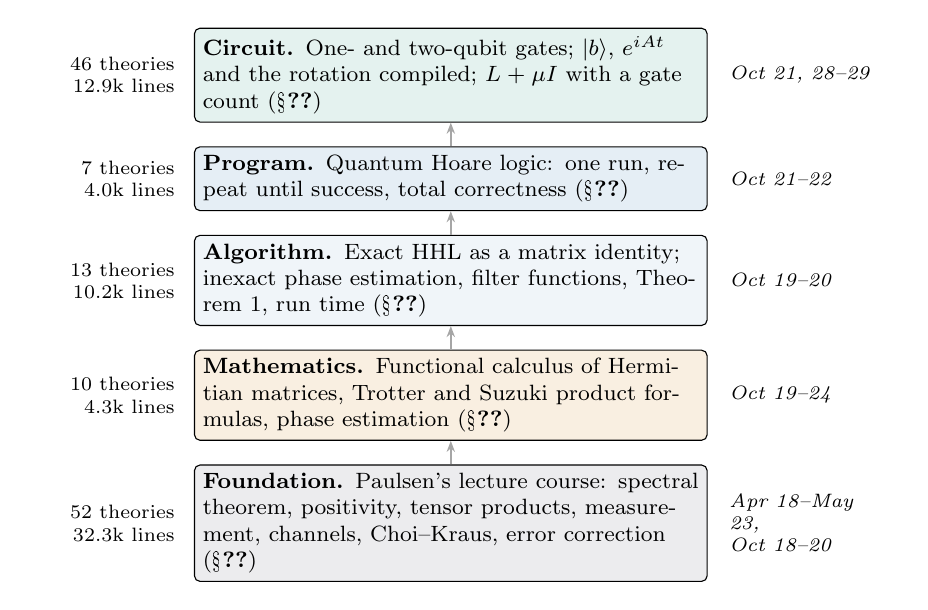
\begin{tikzpicture}[font=\footnotesize,
  lay/.style={draw, rounded corners=2pt, text width=6.3cm, align=left, inner sep=3pt},
  when/.style={font=\scriptsize\itshape, text width=2.05cm, align=left, anchor=west},
  size/.style={font=\scriptsize, text width=1.75cm, align=right, anchor=east},
  arr/.style={-{Stealth[length=4pt]}, thick, gray!70}]
\node[lay, fill=notes!14] (L0) {\textbf{Foundation.} Paulsen's lecture course: spectral theorem, positivity,
  tensor products, measurement, channels, Choi--Kraus, error correction (\S\ref{sec:foundation})};
\node[lay, fill=hfc!14, above=0.3cm of L0] (L1) {\textbf{Mathematics.} Functional calculus of Hermitian matrices,
  Trotter and Suzuki product formulas, phase estimation (\S\ref{sec:math})};
\node[lay, fill=hhl!7, above=0.3cm of L1] (L2) {\textbf{Algorithm.} Exact HHL as a matrix identity; inexact
  phase estimation, filter functions, Theorem~1, run time (\S\ref{sec:algorithm})};
\node[lay, fill=hhl!12, above=0.3cm of L2] (L3) {\textbf{Program.} Quantum Hoare logic: one run, repeat until
  success, total correctness (\S\ref{sec:programs})};
\node[lay, fill=gates!12, above=0.3cm of L3] (L4) {\textbf{Circuit.} One- and two-qubit gates; $\ket b$, $e^{iAt}$
  and the rotation compiled; $L+\mu I$ with a gate count (\S\ref{sec:gates})};
\foreach \a/\b in {L0/L1, L1/L2, L2/L3, L3/L4} \draw[arr] (\a.north) -- (\b.south);
\node[when] at ($(L4.east)+(0.15,0)$) {Oct 21, 28--29};
\node[when] at ($(L3.east)+(0.15,0)$) {Oct 21--22};
\node[when] at ($(L2.east)+(0.15,0)$) {Oct 19--20};
\node[when] at ($(L1.east)+(0.15,0)$) {Oct 19--24};
\node[when] at ($(L0.east)+(0.15,0)$) {Apr 18--May 23,\\ Oct 18--20};
\node[size] at ($(L4.west)+(-0.12,0)$) {46 theories\\ 12.9k lines};
\node[size] at ($(L3.west)+(-0.12,0)$) {7 theories\\ 4.0k lines};
\node[size] at ($(L2.west)+(-0.12,0)$) {13 theories\\ 10.2k lines};
\node[size] at ($(L1.west)+(-0.12,0)$) {10 theories\\ 4.3k lines};
\node[size] at ($(L0.west)+(-0.12,0)$) {52 theories\\ 32.3k lines};
\end{tikzpicture}
\caption{The verified stack. Each level is proved from the one below; left, the size of each level in
the final development; right, the days on which it was built. The foundation was written in spring; everything above it was written after a pause of
almost five months, in eleven days of October 2026.}\label{fig:stack}
\end{figure}

\paragraph{How it was built.} The second subject of this paper is the process. The development was
written by an AI coding agent, Claude Code~\cite{claudecode}, under the direction of one
mathematician, the author, who wrote almost no proof text himself. It was not built in one sprint. A
formalisation of Vern Paulsen's lecture course on quantum computing and completely positive
maps~\cite{paulsen2011notes} was written in April and May 2026; then nothing happened for 147 days;
then, in eleven days of October, the course was completed and HHL was verified on top of it, from
the first theorem about phase estimation to the gate-level pipeline. Following the example of Ilin's
report on a Lean formalisation in plasma physics~\cite{ilin2026vml}, we report the timeline, the
statistics recoverable from the repository and the agent's logs, the role of the human, the ways in
which the agent failed, and what we learned. Our setting differs from his in three ways: the target
is a published algorithm whose paper turned out to contain errors, the work is split by a long
pause, and it builds on an earlier formalisation by the same team, which makes it a case study in
how an agent-built library ages and is reused.

\paragraph{Contributions.}
\begin{itemize}
\item A verification of HHL at four levels: mathematics, algorithm, program and circuit
(Sections~\ref{sec:hhl}--\ref{sec:results}). It includes total correctness of the repeat-until-success
loop, which needs a new proof rule for loops with a resetting body, the paper's error analysis with
explicit constants, and a gate-level pipeline with a closed-form gate count.
\item Errata to the HHL paper, each backed by a formal counterexample or a corrected theorem
(Section~\ref{sec:errata}).
\item A quantitative account of an agent-built formalisation that spans a long pause: 571 commits,
34 active days, 238 prompts in October, almost ten thousand tool calls, and the evolution of the
human's role from proving lemmas to judging statements, names and presentation
(Section~\ref{sec:process}).
\item Lessons on verifying quantum algorithms and on formalising with an agent, among them
the failure modes we observed and the checks that caught them (Section~\ref{sec:lessons}).
\end{itemize}

All results are checked by Isabelle2026 with \texttt{quick\_and\_dirty = false}, so no
\texttt{sorry} survives. An audit with \isa{Thm\_Deps.all\_oracles} over every theorem finds one
oracle, the Types-To-Sets rule \isa{cancel\_type\_definition}, and only in two side sessions, which
inherit it from imported AFP entries (Section~\ref{sec:trust}). The development is organised as
three entries for the Archive of Formal Proofs (AFP). The sources, the documents and the audits are
in the project repository;\footnote{\url{https://github.com/brydustin/Quantum_Computing}, commit
\texttt{1e37476}.} each listing below links to its source line (\isalogo).

\section{HHL and Quantum Hoare Logic}\label{sec:hhl}

\subsection{The Algorithm}

Write $A=\sum_j\lambda_j\ketbra{u_j}{u_j}$ and $\ket b=\sum_j\beta_j\ket{u_j}$. Phase estimation with
the unitaries $e^{iAt_0}$ writes an approximation $\tilde\lambda_j$ of each eigenvalue into a clock
register, which gives $\sum_j\beta_j\ket{\tilde\lambda_j}\ket{u_j}$. A rotation of an ancilla qubit,
controlled by the clock, produces the amplitudes $C/\tilde\lambda_j$. Uncomputing the clock and
measuring the ancilla leaves, on outcome~$1$, the state $\sum_j(\beta_j/\lambda_j)\ket{u_j}$, which is
$A^{-1}\ket b$ up to normalisation. The success probability is $p=C^2\norm{A^{-1}b}^2$, at least
$1/\kappa^2$ for $C=\lambda_{\min}$ and unit~$b$, so the measurement is repeated or amplified.
Figure~\ref{fig:hhl} shows the circuit together with the state after each gate, which is itself a
theorem of the development.

\begin{figure}[t]
\centering
\scalebox{0.8}{%
\begin{quantikz}[row sep={0.8cm,between origins}, column sep=0.2cm]
\lstick{clock $\ket{0}^{\otimes k}$} & \qwbundle{k} &  & \gate{H^{\otimes k}}\slice{$\psi_2$}
  & \ctrl{1}\slice{$\psi_3$} & \gate{F^\dagger}\slice{$\psi_4$} & \ctrl{2}\slice{$\psi_5$}
  & \gate{F}\slice{$\psi_6$} & \ctrl{1}\slice{$\psi_7$} & \gate{H^{\otimes k}}\slice{$\psi_8$} & \\
\lstick{system $\ket{0}^{\otimes s}$} & \qwbundle{s} & \gate{U_b}\slice{$\psi_1$} & & \gate{U^{c}}
  & & & & \gate{U^{-c}} & & \rstick{$\propto A^{-1}b$ if $1$}\\
\lstick{ancilla $\ket0$} & & & & & & \gate{R(C/\lambda_c)} & & & & \meter{}
\end{quantikz}}
\\[0.6em]
\renewcommand{\arraystretch}{1.15}\small
\begin{tabular}{@{}l@{\enspace}l@{\qquad}l@{\enspace}l@{}}
$\psi_1$ & $\ket0\otimes b\otimes\ket0$ &
$\psi_5$ & $\sum_j\ket j\otimes\Pi_jb\otimes R(C/\lambda_j)\ket0$\\
$\psi_2$ & $u\otimes b\otimes\ket0$ &
$\psi_6$ & $\sum_j\ket j\otimes N^{-1/2}(U^{j}\otimes I)\,w$\\
$\psi_3$ & $\sum_j\ket j\otimes N^{-1/2}U^{j}b\otimes\ket0$ &
$\psi_7$ & $u\otimes w$\\
$\psi_4$ & $\sum_j\ket j\otimes\Pi_jb\otimes\ket0$ &
$\psi_8$ & $\ket0\otimes w$
\end{tabular}\\[0.2em]
{\small $w=\sqrt{I-C^2A^{-2}}\,b\otimes\ket0+CA^{-1}b\otimes\ket1$}
\caption{The HHL circuit and the state after each of its eight gates, from $\ket0\ket0\ket0$, for
$N=2^k$, $U=e^{iAt_0}$, $u=N^{-1/2}\sum_j\ket j$ and every eigenvalue of $A$ on the grid
$\lambda_j=2\pi j/(Nt_0)$ (read as $2\pi(j-N)/(Nt_0)$ for $j\ge N/2$). Gate~3 applies $U^c$ when the
clock holds $c$, gate~5 applies $R(C/\lambda_c)$ with $R(c)\ket0=\sqrt{1-c^2}\ket0+c\ket1$, and $\Pi_j$
is the spectral projector of $A$ at $\lambda_j$. The table is the theorem \isa{hhl\_steps}.}\label{fig:hhl}
\end{figure}

\subsection{Programs and Triples}

We use the concrete matrices of the Jordan-Normal-Form library~\cite{thiemann2015jnf}, shared by
\IMD~\cite{bordg2021imd,bordg2020afp}, the quantum Fourier transform entry~\cite{manrique2025qft} and
QHLProver~\cite{liu2019qhl,liu2019afp}. Dimensions are hypotheses (\isa{A $\in$ carrier\_mat n n})
rather than types, which is how the physics literature treats them and lets the libraries share
their definitions. QHLProver formalises Ying's quantum while-language~\cite{ying2011,ying2016book},
\[
S \;::=\; \mathbf{skip} \;\mid\; U \;\mid\; S_1;S_2 \;\mid\; \mathbf{measure}\ M\ [S_0,\dots,S_{m-1}]
\;\mid\; \mathbf{while}\ M\ \mathbf{do}\ S ,
\]
whose programs denote completely positive, trace-non-increasing maps on partial density operators;
the trace lost by a loop is the probability that it does not terminate. A predicate is an operator
$0\le P\le I$, and $\Tr(P\rho)$ is the probability that $P$ holds in the state~$\rho$. A triple
compares these probabilities before and after the program (Listing~\ref{lst:triples}).

\begin{lstlisting}[float=tp,caption={Triples in QHLProver (in the locale \isa{state\_sig} of the registers, of
total dimension \isa{d}; syntax annotations omitted)},label={lst:triples}]
definition hoare_total_correct :: "complex mat ~$\Rightarrow$~ com ~$\Rightarrow$~ complex mat
    ~$\Rightarrow$~ bool" where
  "~$\models_{t}$~ {P} S {Q} ~$\longleftrightarrow$~ (~$\forall\rho\in$~density_states. trace (P * ~$\rho$~) ~$\le$~ trace (Q *
      denote S ~$\rho$~))"
definition hoare_partial_correct :: "complex mat ~$\Rightarrow$~ com ~$\Rightarrow$~ complex
    mat ~$\Rightarrow$~ bool" where
  "~$\models_{p}$~ {P} S {Q} ~$\longleftrightarrow$~ (~$\forall\rho\in$~density_states.
      trace (P * ~$\rho$~) ~$\le$~ trace (Q * denote S ~$\rho$~) + (trace ~$\rho$~ - trace
          (denote S ~$\rho$~)))"
\end{lstlisting}

Every statement about HHL below is a triple of one of four shapes (Table~\ref{tab:readings}). Let
$P_0$, $P_1$ project onto ancilla value $0$, $1$, and let $\ket t$ be a unit vector with
$P_1\ket t=\ket t$. Since $\Tr\rho=1$ for a state, a precondition $q\cdot I$ asserts the number $q$ for
every input. The second reading needs a line of argument: if $\Tr((P_0+\ketbra tt)\sigma)\ge1$ for
$\sigma=\sem S\rho$, then $\Tr((P_1-\ketbra tt)\sigma)\le0$, and since $P_1-\ketbra tt\ge0$, the
ancilla can only read $1$ in the state $\ket t$.

\begin{table}[t]
\caption{The four shapes of triple used for HHL, for a state $\rho$ with $\Tr\rho=1$.}\label{tab:readings}
\centering\small
\begin{tabular}{@{}l>{\raggedright\arraybackslash}p{6.9cm}@{}}
\toprule
Triple & Reading\\
\midrule
$\hoaret{p\cdot I}{S}{P_1}$ & $S$ ends with the ancilla in $\ket1$ with probability at least $p$\\
$\hoaret{I}{S}{P_0+\ketbra tt}$ & whenever the ancilla reads $1$ at the end, the state is exactly $\ket t$\\
$\hoaret{I}{S}{\ketbra tt}$ & $S$ terminates with probability one, in the state $\ket t$\\
$\hoaret{q\cdot I}{S}{\ketbra tt}$ & the output has fidelity at least $q$ with $\ket t$\\
\bottomrule
\end{tabular}
\end{table}

Section~\ref{sec:programs} presents the proof system with which such triples are derived, the rules
we added to it for algorithms, and the triples of phase estimation and HHL.

\section{The Verified Algorithm, Level by Level}\label{sec:results}

This section follows Fig.~\ref{fig:stack} from the bottom. Each major result is stated informally
first and then as the Isabelle text, copied from the sources and checked against them
mechanically (Appendix~\ref{app:method}).

\subsection{The Foundation}\label{sec:foundation}

Vern Paulsen's course \emph{Lectures on Quantum Computing and Completely Positive
Maps}~\cite{paulsen2011notes}, given in Houston in 2011, runs over 34 lectures from Hilbert spaces to
quantum error correction. Its formalisation follows the lectures in order, in 46 theories, on top of
a session of reusable matrix analysis, and every definition and theorem of the notes was audited
against the formal text. The audit found false statements in the notes, each witnessed formally:
the Day~29 ``Hamming $[7,1,3]$'' code has distance~2 and corrects no error
(\isa{notes\_hamming\_not\_correcting}), and on Day~32 two Pauli errors that the notes call
distinguishable agree on the Shor code space (\isa{shor\_notes\_Z1\_Z2}). For HHL, the first ten
lectures matter most: the spectral theorem, positivity and square roots, tensor products and
measurement. The later lectures give the meaning of quantum programs: Choi's theorem
(Listing~\ref{lst:choi}) characterises completely positive maps, which is what a quantum program
denotes, and a theory of the HHL entry reads off Kraus operators from any loop-free program and proves
the program a channel.

Two bridges connect the lectures to the rest of the AFP. Formalising a lecture course means
defining what the course defines, so the notes have their own Hermitian, positive semidefinite and
density matrices; the theory \isa{Notes\_Library\_Bridge} proves each equal to its counterpart in
QHLProver and \IMD{} (\isa{psd\_AFP}: \isa{psd P $\longleftrightarrow$ positive P}). The session
\isa{Kraus\_Maps\_Bridge} connects the course to Unruh's \emph{Kraus Maps}
entry~\cite{unruh2025kraus}, which develops Kraus maps on trace-class operators of arbitrary Hilbert
spaces but does not prove Choi's theorem. For finite types the two settings meet: a list of Kraus
matrices becomes a Kraus family whose map is the lectures' $\rho\mapsto\sum_iW_i\rho W_i^\dagger$, and
with the lectures' Choi theorem every completely positive map in Paulsen's sense is a Kraus map of the
library (Fig.~\ref{fig:krausbridge}, Listing~\ref{lst:choi}).

\begin{figure}[t]
\centering
\begin{tikzcd}[column sep=12.5em, row sep=3.6em, cells={font=\small},
  every label/.append style={font=\footnotesize}]
\rho\in\C^{n\times n} \arrow[r, "\rho\;\mapsto\;\textstyle\sum_iW_i\rho W_i^\dagger"] \arrow[d, "\mathit{tc\_of\_mat}"']
  & \C^{d\times d} \\
T_\rho\in\mathcal T(\ell^2(\alpha)) \arrow[r, "\mathit{kf\_apply}\;(\mathit{kf\_of\_mats}\;\mathit{Ws})"', shorten=4pt]
  & \mathcal T(\ell^2(\beta)) \arrow[u, "\mathit{mat\_of\_tc}"']
\end{tikzcd}
\caption{The bridge to \emph{Kraus Maps} as a commuting square (\isa{kf\_of\_mats\_apply}): for finite types
$\alpha$, $\beta$ of sizes $n$ and $d$, the lectures' Kraus map on matrices (top) agrees with Unruh's Kraus map
on trace-class operators (bottom), read through the translation between matrices and operators. With
Choi's theorem it follows that every completely positive map of the lectures is a Kraus map of the
library (\isa{cp\_kraus\_map}).}\label{fig:krausbridge}
\end{figure}

%%LST Day19_Choi_Theorem.thy choi_theorem ; Kraus_Maps_Bridge/Kraus_Maps_Bridge.thy cp_kraus_map
\begin{lstlisting}[float=tp,caption={Choi's theorem (Lecture 19), and the lectures' completely positive maps as Kraus maps of the AFP entry \emph{Kraus Maps}; \isa{tc\_map} reads a map of matrices as a map of trace-class operators on \isa{'a ell2}},label={lst:choi}]
theorem choi_theorem:
  fixes ~$\Phi$~ :: "complex Matrix.mat ~$\Rightarrow$~ complex Matrix.mat"
  assumes linear: "~$\bigwedge$~A B. A ~$\in$~ carrier_mat n n ~$\Longrightarrow$~ B ~$\in$~ carrier_mat n n
      ~$\Longrightarrow$~ ~$\Phi$~ (A + B) = ~$\Phi$~ A + ~$\Phi$~ B"
    and smult: "~$\bigwedge$~c A. A ~$\in$~ carrier_mat n n ~$\Longrightarrow$~ ~$\Phi$~ (c ~$\cdot_{m}$~ A) = c ~$\cdot_{m}$~ ~$\Phi$~ A"
    and range: "~$\forall$~A. A ~$\in$~ carrier_mat n n ~$\longrightarrow$~ ~$\Phi$~ A ~$\in$~ carrier_mat d d"
    and npos: "n > 0"
    and dpos: "d > 0"
  shows "completely_positive n d ~$\Phi$~ ~$\longleftrightarrow$~ psd (choi_matrix n d ~$\Phi$~)"
theorem cp_kraus_map:
  fixes ~$\Phi$~ :: "complex Matrix.mat ~$\Rightarrow$~ complex Matrix.mat"
  assumes linear: "~$\bigwedge$~A B. A ~$\in$~ carrier_mat CARD('a) CARD('a) ~$\Longrightarrow$~ B ~$\in$~
      carrier_mat CARD('a) CARD('a) ~$\Longrightarrow$~ ~$\Phi$~ (A + B) = ~$\Phi$~ A + ~$\Phi$~ B"
    and smult: "~$\bigwedge$~c A. A ~$\in$~ carrier_mat CARD('a) CARD('a) ~$\Longrightarrow$~ ~$\Phi$~ (c ~$\cdot_{m}$~ A)
        = c ~$\cdot_{m}$~ ~$\Phi$~ A"
    and range: "~$\forall$~A. A ~$\in$~ carrier_mat CARD('a) CARD('a) ~$\longrightarrow$~ ~$\Phi$~ A ~$\in$~
        carrier_mat CARD('b) CARD('b)"
    and cp: "completely_positive CARD('a) CARD('b) ~$\Phi$~"
  shows "Kraus_Maps.kraus_map (tc_map ~$\Phi$~ :: ('a::enum ell2, 'a ell2)
      trace_class ~$\Rightarrow$~ ('b::enum ell2, 'b ell2) trace_class)"
\end{lstlisting}

\subsection{Mathematics}\label{sec:math}

\paragraph{A functional calculus.} HHL computes $A^{-1}$, $e^{iAt}$ and $\sqrt{I-C^2A^{-2}}$ of a
Hermitian matrix, so its proof needs $g(A)$ for real functions~$g$. We define $g(A)$ by what it does
to eigenvectors rather than through a chosen diagonalisation.

\begin{theorem}[functional calculus]\label{thm:matfun}
Let $A\in\C^{n\times n}$ be Hermitian. There is exactly one matrix $g(A)$ with $g(A)v=g(\lambda)v$ for
every eigenvector $v$ of $A$ with eigenvalue~$\lambda$, and $g(A)=U\operatorname{diag}(g(d_1),\dots,g(d_n))
U^\dagger$ for every spectral decomposition $U^\dagger AU=\operatorname{diag}(d_1,\dots,d_n)$.\isalink{Hermitian_Functional_Calculus/Hermitian_Functional_Calculus.thy}{497}
\end{theorem}

%%LST Hermitian_Functional_Calculus/Hermitian_Functional_Calculus.thy acts_on_eigenvectors mat_fun_unique
\begin{lstlisting}[float=tp,caption={The functional calculus: \isa{B acts\_as g on\_eigenvectors\_of A} is notation for \isa{acts\_on\_eigenvectors A g B}, and \isa{mat\_fun g A} is the unique such \isa{B}},label={lst:matfun}]
definition acts_on_eigenvectors :: "complex Matrix.mat ~$\Rightarrow$~ (real ~$\Rightarrow$~
    complex) ~$\Rightarrow$~ complex Matrix.mat ~$\Rightarrow$~ bool" where
  "acts_on_eigenvectors A g B ~$\longleftrightarrow$~ (~$\forall$~v l. dim_vec v = dim_row A ~$\longrightarrow$~ A *~$_{v}$~
      v = complex_of_real l ~$\cdot_{v}$~ v ~$\longrightarrow$~ B *~$_{v}$~ v = g l ~$\cdot_{v}$~ v)"
corollary mat_fun_unique:
  assumes A: "A ~$\in$~ carrier_mat n n" "hermitian A"
  shows "~$\exists$~!B. B ~$\in$~ carrier_mat n n ~$\wedge$~ B acts_as g on_eigenvectors_of A"
\end{lstlisting}

The definition makes the algebra of the calculus short: two matrices that agree on all
eigenvectors of~$A$ are equal, because the eigenvectors span, so identities such as
$g(A)h(A)=(gh)(A)$ and $g(A)^\dagger=\bar g(A)$ need no sums over an eigenbasis. The same principle
proves HHL itself (Section~\ref{sec:algorithm}). On top of the calculus we verify the Lie--Trotter
formula with an explicit bound,
\[
\norm{(e^{itH_1/r}\cdots e^{itH_m/r})^r-e^{it(H_1+\dots+H_m)}}\le2(mLt)^2/r
\]
for Hermitian $H_j$ of norm at most~$L$, and Suzuki's higher-order formulas with error of order
$|t|^{2k+3}/r^{2k+2}$.\isalink{Hermitian_Functional_Calculus/Trotter_Product_Formula.thy}{612}

\paragraph{Phase estimation.} Phase estimation is HHL's engine. With $F_N$ the Fourier matrix and
$\Lambda(U)=\sum_k\ketbra kk\otimes U^k$:

\begin{theorem}[phase estimation]\label{thm:qpe}
If $Uv=e^{2\pi i\varphi}v$, then $(F_N^\dagger\otimes I)\Lambda(U)(u\otimes v)=(\sum_j\alpha_j\ket
j)\otimes v$ with $\alpha_j=\frac1N\sum_{k<N}e^{2\pi ik(\varphi-j/N)}$. If $\varphi=j_0/N$, then
$\alpha=\ket{j_0}$. If $|\varphi-j/N|\le1/(2N)$, then $|\alpha_j|^2\ge4/\pi^2$.\isalink{Algorithms/Phase_Estimation.thy}{287}
\end{theorem}

%%LST Algorithms/Phase_Estimation.thy phase_estimation phase_estimation_bound
\begin{lstlisting}[float=tp,caption={Phase estimation and the $4/\pi^2$ bound},label={lst:qpe}]
theorem phase_estimation:
  assumes U: "U ~$\in$~ carrier_mat m m" and u: "dim_vec u = m"
    and ev: "U *~$_{v}$~ u = cis (2 * pi * ~$\varphi$~) ~$\cdot_{v}$~ u"
  shows "(((fourier N)~$^{\dagger}$~) ~$\otimes$~ 1~$_{m}$~ m) *~$_{v}$~ (ctrl_pow N m U *~$_{v}$~ tensor_vec
      (uniform_state N) u) = tensor_vec (Matrix.vec N (pe_amp N ~$\varphi$~)) u"
theorem phase_estimation_bound:
  assumes N: "0 < N" and close: "~$|\varphi$~ - real j / real N~$|$~ ~$\le$~ 1 / (2 * real
      N)"
  shows "4 / pi~$^{2}$~ ~$\le$~ (cmod (pe_amp N ~$\varphi$~ j))~$^{2}$~"
\end{lstlisting}

We also prove that the Fourier circuit of the AFP entry~\cite{manrique2025qft} computes $F_N$, so
the theorem holds for an actual circuit, and the textbook precision bound: with
$n+\lceil\log_2(2+1/(2\varepsilon))\rceil$ clock qubits the estimate is within $2^{-n}$ with probability
at least $1-\varepsilon$~\cite{nielsenchuang}. As a program, phase estimation satisfies, for every set
$J$ of clock values, the triple $\hoaret{(\sum_{j\in J}|\alpha_j|^2)\,I}{\mathit{QPE}}{\Pi_J}$, whose
precondition is the weakest possible.

\begin{figure}[t]
\centering
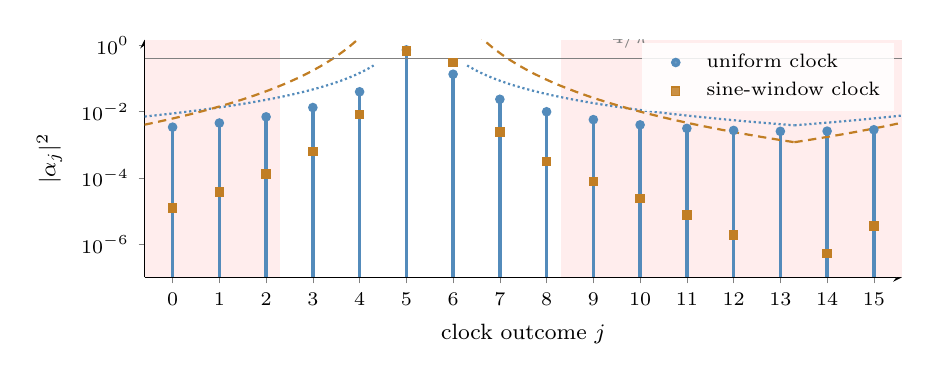
\begin{tikzpicture}
\begin{axis}[width=11.2cm, height=4.6cm, ymode=log, log origin y=infty, ymin=1e-7, ymax=1.5,
  xmin=-0.6, xmax=15.6, axis lines=left, xtick={0,...,15}, ytick={1e-6,1e-4,1e-2,1},
  xlabel={clock outcome $j$}, ylabel={$|\alpha_j|^2$}, tick label style={font=\scriptsize},
  label style={font=\footnotesize}, legend style={font=\scriptsize, draw=none, fill=white, fill opacity=0.85,
  text opacity=1, at={(0.99,0.99)}, anchor=north east}, legend cell align=left]
\fill[red!7] (axis cs:-0.6,1e-7) rectangle (axis cs:2.3,1.5);
\fill[red!7] (axis cs:8.3,1e-7) rectangle (axis cs:15.6,1.5);
\addplot[ycomb, very thick, hhl!80, mark=*, mark size=1.1pt] coordinates
  {(0,0.003435) (1,0.004576) (2,0.007018) (3,0.01342) (4,0.0401) (5,0.7377) (6,0.1362) (7,0.02382)
   (8,0.009999) (9,0.005794) (10,0.004022) (11,0.003158) (12,0.002731) (13,0.002566) (14,0.002606) (15,0.002864)};
\addlegendentry{uniform clock}
\addplot[only marks, hfc!90!black, mark=square*, mark size=1.5pt] coordinates
  {(0,1.228e-05) (1,3.794e-05) (2,0.0001311) (3,0.0006419) (4,0.008282) (5,0.6851) (6,0.3029) (7,0.002423)
   (8,0.0003187) (9,7.778e-05) (10,2.41e-05) (11,7.718e-06) (12,1.925e-06) (13,9.227e-08) (14,5.157e-07) (15,3.57e-06)};
\addlegendentry{sine-window clock}
\addplot[densely dotted, thick, hhl!80, domain=-0.6:4.3, samples=40, forget plot] {1/(4*(5.3-x)^2)};
\addplot[densely dotted, thick, hhl!80, domain=6.3:13.3, samples=40, forget plot] {1/(4*(x-5.3)^2)};
\addplot[densely dotted, thick, hhl!80, domain=13.3:15.6, samples=10, forget plot] {1/(4*(21.3-x)^2)};
\addplot[densely dashed, thick, hfc!90!black, domain=-0.6:4.3, samples=40, forget plot] {pi^2/(2*(5.3-x)^4)};
\addplot[densely dashed, thick, hfc!90!black, domain=6.3:13.3, samples=40, forget plot] {pi^2/(2*(x-5.3)^4)};
\addplot[densely dashed, thick, hfc!90!black, domain=13.3:15.6, samples=10, forget plot] {pi^2/(2*(21.3-x)^4)};
\addplot[gray, domain=-0.6:15.6, samples=2, forget plot] {4/pi^2};
\node[font=\scriptsize, gray, anchor=south west] at (axis cs:9.2,0.42) {$4/\pi^2$};
\end{axis}
\end{tikzpicture}
\caption{The outcome distribution of phase estimation for $N=16$ and $N\varphi=5.3$ (logarithmic scale),
computed from the definitions, with the two clock states. The nearest outcome has probability at least
$4/\pi^2$ (Theorem~\ref{thm:qpe}). Away from it, the uniform clock's amplitudes obey only
$|\alpha_j|^2\le1/(4N^2\delta_j^2)$ (dotted, \isa{pe\_amp\_tail}), the window's obey
$|\alpha_j|^2\le\pi^2/(2N^4\delta_j^4)$ (dashed, \isa{win\_amp\_tail}). The outcomes more than three
steps from $N\varphi$ (shaded) have total probability $0.039$ with the uniform clock and $0.0003$ with
the window: this is why the window makes $N\sim1/\varepsilon$ enough (Theorem~\ref{thm:window}).}\label{fig:qpe}
\end{figure}

\subsection{The Algorithm}\label{sec:algorithm}

\paragraph{Exact HHL.} Let $W=(F^\dagger\otimes I)\,\Lambda(U)$ be phase estimation without its
input, and $R$ the clock-controlled rotation.

\begin{theorem}[exact HHL]\label{thm:hhl}
Let $A\in\C^{n\times n}$ be Hermitian with every eigenvalue a grid value $\lambda_k$, $0<k<N$. Then
for every $b\in\C^n$ and every real $C$,
\[
W^\dagger RW\,(u\otimes b\otimes\ket0)=u\otimes\bigl(\sqrt{I-C^2A^{-2}}\,b\otimes\ket0+CA^{-1}b\otimes\ket1\bigr).
\]
Hence the ancilla reads $1$ with probability $C^2\norm{A^{-1}b}^2$, and if $C\le|\lambda|\le\Lambda$ on
the spectrum, this is at least $(C/\Lambda)^2\norm b^2$, which is $1/\kappa^2$ for unit
$b$ and $C=\lambda_{\min}$.\isalink{Algorithms/HHL.thy}{590}
\end{theorem}

%%LST Algorithms/HHL.thy hhl
\begin{lstlisting}[float=tp,caption={Exact HHL as a matrix identity, for every right-hand side},label={lst:hhl}]
theorem hhl:
  assumes A: "A ~$\in$~ carrier_mat n n" "hermitian A" and t0: "0 < t0" and
      N: "0 < N"
    and spec: "~$\bigwedge$~l. l ~$\in$~ herm_spectrum A ~$\Longrightarrow$~ ~$\exists$~k. 0 < k ~$\wedge$~ k < N ~$\wedge$~ l =
        reg_eig t0 N k"
    and b: "dim_vec b = n"
  shows "hhl_circuit A t0 N C *~$_{v}$~ tensor_vec (uniform_state N)
      (tensor_vec b (unit_vec 2 0)) = tensor_vec (uniform_state N)
      (tensor_vec (mat_fun (~$\lambda$~x. complex_of_real (sqrt (1 - (C / x)~$^{2}$~)))
      A *~$_{v}$~ b) (unit_vec 2 0) + tensor_vec ((complex_of_real C ~$\cdot_{m}$~
      herm_inv A) *~$_{v}$~ b) (unit_vec 2 1))"
\end{lstlisting}

The proof is the eigenvector principle again. On an eigenvector $v$ of $A$ with eigenvalue
$\lambda_k$, phase estimation writes $\ket k$ exactly, the rotation multiplies by
$R(C/\lambda_k)$, and uncomputation restores the clock; both sides of the identity are linear in $b$
and agree on eigenvectors, so they agree everywhere. No eigenbasis expansion of $b$ appears anywhere
in the proof, although every textbook account is written as one.

\paragraph{Inexact HHL.} The paper's error analysis drops the grid assumption. If $\lambda$ is not a
grid value, phase estimation spreads each eigenvector over the clock, the rotation acts on every
branch with its own angle, and uncomputation is inexact. Branches are orthogonal, which gives an exact
identity for the error on an eigenvector, and the errors of distinct eigenvectors are orthogonal too, so
the bound extends to every $b$ without a dependence on the dimension. Everything then depends on how fast
the clock amplitudes decay away from the true phase. With the uniform clock state they decay like
$1/(N\delta)$, which would need $N\sim1/\varepsilon^2$; the paper prepares the clock in a sine window
instead, whose amplitudes decay like $1/(N\delta)^2$ (Fig.~\ref{fig:qpe}).

\begin{theorem}[window register]\label{thm:window}
Let $0<C$ and $0<\theta<1$, and let $A$ be Hermitian with every eigenvalue in the
interval from $\lambda_{\min}\ge2C/\theta$ to $\pi/(2t_0)$. For every $b$, the circuit with the sine-window clock and the rotation clamped
to $[-1,1]$ satisfies
\[
\norm{\mathrm{out}-\psi\otimes w}^2\le\Bigl(\frac{K_1}{N^2}+\frac{K_2}{N^3}\Bigr)\norm b^2,
\]
with $K_1=8\pi^2(2+\pi^2)\theta^4/(t_0^2C^2(1-\theta^2))$ and $K_2=512\pi^6/(t_0^4\lambda_{\min}^4)$,
where $\psi$ is the window state and $w$ the exact output of Theorem~\ref{thm:hhl}. Hence a clock of size
$N\sim1/\varepsilon$ gives error at most $\varepsilon\norm b$.\isalink{Algorithms/HHL_Window.thy}{739}
\end{theorem}

The paper's own analysis also flags ill-conditioned eigenvalues instead of inverting them. Its
\emph{filter functions} $f$, $g$ (Fig.~\ref{fig:filters}) send an eigenvalue to a flag state
$\ket{h(\lambda)}=\sqrt{1-f^2-g^2}\ket{\mathit{nothing}}+f\ket{\mathit{well}}+g\ket{\mathit{ill}}$, and the
paper's Theorem~1 bounds the error of the flagged output in terms of the total evolution time $t=Nt_0$.

\begin{theorem}[Theorem~1 of the HHL paper, with constants]\label{thm:thm1}
Let $A$ be Hermitian with $|t_0\lambda|\le\pi/2$ on its spectrum, let the flag gates prepare
$\ket{h(\tilde\lambda_k)}$ for each clock value~$k$, and let $c=\pi^2\sqrt{4+2\pi^2}$. For every $b$, the
flagged output is within $3c\,\kappa\norm b/t$ of the ideal one, and the states post-selected on
$\{\mathit{well},\mathit{ill}\}$ (or on $\mathit{well}$, for $b$ in the well-conditioned subspace) are within
$12c\,\kappa/t$ of the ideal ones.\isalink{Algorithms/HHL_Filter_Bounds.thy}{330}
\end{theorem}

\begin{theorem}[run time]\label{thm:runtime}
Let the spectrum of $A$ lie in $[1/\kappa,1]$, let $t_0\le\pi/2$, $\varepsilon\kappa\le1$ and
$Nt_0\ge12c\,\kappa/\varepsilon$, and let $\norm b=1$. Then the post-selected output is within
$\varepsilon$ of $\psi\otimes A^{-1}b/\norm{A^{-1}b}\otimes\ket{\mathit{well}}$, its amplitude is at least
$1/(4\kappa)$, and amplitude amplification with $k\le\pi\kappa$ rounds and $(2k+1)\cdot2(N-1)$ calls of the
evolution succeeds with probability at least $1-\norm y^2$, where $y$ is the post-selected part of
one run.\isalink{Algorithms/HHL_Runtime.thy}{302}
\end{theorem}

\noindent An oracle $V$ with $\norm{Vv-e^{iAt_0}v}\le\eta\norm v$ moves every output by at most the number
of calls times~$\eta$, so the theorems hold for a simulated evolution with an additional error
$2(N-1)\eta$. The rest of the paper is verified too: the reduction from circuits to matrix inversion
behind its optimality theorems (with $\kappa\le2T+1$ for a circuit of $T$ gates), rectangular and
preconditioned systems, and the estimation of $\langle x|M|x\rangle$ from samples. Several of its
statements turned out to be false (Section~\ref{sec:errata}).

\section{What the Formalisation Found}\label{sec:errata}

The HHL paper is a short letter with a long appendix, and its main claims survive mechanisation; they
are stated with $O(\cdot)$ and hold with other constants. Its details do not all survive.
Table~\ref{tab:errata} lists the statements of the arXiv version~\cite{hhl2008arxiv} that are false as
written, each with the correction and the formal theorem that refutes the claim or proves the
correction. Most sit in the appendix on optimality, which reduces quantum circuits to matrix
inversion; each optimality theorem is formalised up to the complexity-theoretic fact it cites.

The most instructive is Lemma~3, the Lipschitz estimate behind the paper's Theorem~1. The filter
functions mark an eigenvalue $\lambda$ as well-conditioned ($f$), ill-conditioned ($g$) or in between:
$f(\lambda)=1/(2\kappa\lambda)$ and $g(\lambda)=0$ for $\lambda\ge1/\kappa$, $f=0$ and $g=\frac12$ below
$1/(2\kappa)$, and on $[\frac1{2\kappa},\frac1\kappa)$ they turn through a quarter circle of radius
$\frac12$. Lemma~3 claims
\[
|f(\lambda)-f(\tilde\lambda)|^2+|g(\lambda)-g(\tilde\lambda)|^2\;\le\;c\,\kappa^2(\lambda-\tilde\lambda)^2\bigl(|f(\lambda)|^2+|g(\lambda)|^2\bigr)
\]
with $c=\pi^2/2$. At $\lambda=\frac1{2\kappa}$, $\tilde\lambda=\frac1\kappa$ the left side is $\frac14+\frac14=\frac12$,
while $\kappa^2(\lambda-\tilde\lambda)^2=\frac14$ and $f(\lambda)^2+g(\lambda)^2=\frac14$, so the right side is
$c/16=\pi^2/32<\frac12$, for every~$\kappa$. The constant $c=\pi^2$
holds, and no smaller constant does (Listing~\ref{lst:lemma3}). The paper uses the lemma only inside an
$O(\kappa/t)$ bound, so its Theorem~1 is unaffected; with the corrected constant we prove it with
the explicit constant $12\pi^2\sqrt{4+2\pi^2}$.

%%LST Algorithms/HHL_Filter.thy lemma3_paper_constant lemma3 lemma3_sharp
\begin{lstlisting}[float=tp,caption={Lemma~3 of the HHL paper: the counterexample to the paper's constant, the corrected constant, and its sharpness (for fixed \isa{$\kappa$ > 0}; \isa{filt\_f} and \isa{filt\_g} are the filter functions)},label={lst:lemma3}]
theorem lemma3_paper_constant:
  "pi~$^{2}$~ / 2 * ~$\kappa^{2}$~ * (1 / (2 * ~$\kappa$~) - 1 / ~$\kappa$~)~$^{2}$~ * ((filt_f ~$\kappa$~ (1 / (2 *
      ~$\kappa$~)))~$^{2}$~ + (filt_g ~$\kappa$~ (1 / (2 * ~$\kappa$~)))~$^{2}$~) < (filt_f ~$\kappa$~ (1 / (2 *
      ~$\kappa$~)) - filt_f ~$\kappa$~ (1 / ~$\kappa$~))~$^{2}$~ + (filt_g ~$\kappa$~ (1 / (2 * ~$\kappa$~)) - filt_g
      ~$\kappa$~ (1 / ~$\kappa$~))~$^{2}$~"
theorem lemma3:
  "(filt_f ~$\kappa$~ a - filt_f ~$\kappa$~ b)~$^{2}$~ + (filt_g ~$\kappa$~ a - filt_g ~$\kappa$~ b)~$^{2}$~ ~$\le$~ pi~$^{2}$~
      * ~$\kappa^{2}$~ * (a - b)~$^{2}$~ * ((filt_f ~$\kappa$~ a)~$^{2}$~ + (filt_g ~$\kappa$~ a)~$^{2}$~)"
theorem lemma3_sharp:
  assumes c: "c < pi~$^{2}$~"
  shows "~$\exists$~a b. c * ~$\kappa^{2}$~ * (a - b)~$^{2}$~ * ((filt_f ~$\kappa$~ a)~$^{2}$~ + (filt_g ~$\kappa$~ a)~$^{2}$~)
      < (filt_f ~$\kappa$~ a - filt_f ~$\kappa$~ b)~$^{2}$~ + (filt_g ~$\kappa$~ a - filt_g ~$\kappa$~ b)~$^{2}$~"
\end{lstlisting}

\begin{table}[t]
\caption{Errata in the HHL paper (arXiv:0811.3171v3). ``Formal'' names the theorem that refutes the claim
or proves the correction.}\label{tab:errata}
\centering\scriptsize
\renewcommand{\arraystretch}{1.12}
\newcolumntype{L}[1]{>{\raggedright\arraybackslash}p{#1}}
\begin{tabular}{@{}L{1.3cm}L{2.6cm}L{4.5cm}L{2.75cm}@{}}
\toprule
Where & Claim & Correction & Formal\\
\midrule
Lemma 3 & $c=\pi^2/2$ & false for every $\kappa$; $c=\pi^2$ holds and is sharp & \isa{lemma3\_paper\_constant}, \isa{lemma3}, \isa{lemma3\_sharp}\\
Proof of Thm.~4 & $m=\frac2\delta\log(2n)/\log\log n$ rounds suffice & too few: for $n_0=2^{64}$, $\delta=\frac12$ the bound on $T_m$ still exceeds $n_0$; $m\ge\frac2\delta\ln(2n_0)$ suffices & \isa{paper\_rounds\_insufficient}, \isa{corrected\_rounds}\\
(A34) & the dilation satisfies $\kappa^{-1}I\le A\le I$ & impossible: its diagonal is zero & \isa{herm\_embed\_diag}\\
(A37) & the first qubit of $\vec y$ decides acceptance & the top half of $\vec y$ is always $0$; permuting the dilation fixes it & \isa{first\_half\_perm}, \isa{red\_first\_qubit}\\
Thm.~6(2) & precision $\varepsilon=2^{-n-2}$ & cannot separate counts $C$ and $C+1$ once the clock factor ($\le\frac14$) is included & \isa{paper\_precision\_insufficient}\\
App.~A5 & $1/(3\varepsilon^2)$ samples & too few: $\varepsilon=\frac14$, $p=\frac12$ and $6$ samples fail with probability $\frac{11}{16}$; $3/\varepsilon^2$ suffice & \isa{paper\_sample\_count\_too\_small}, \isa{estimate\_expectation}\\
\S IV & preconditioned system $(AB)c=Bb$ & neither left nor right preconditioning: in a $2\times2$ example its solution gives no solution of $Ax=b$ & \isa{paper\_precondition\_wrong}\\
App.~A5 & undo gates $U^\dagger_{3T+1-t}$ & must be $U^\dagger_{T+1-t}$ & construction \isa{red\_U}, \isa{red\_inverse}\\
App.~A5 & $\kappa\le2T$ & we prove $\kappa\le2T+1$ & \isa{red\_A\_bounds}\\
\bottomrule
\end{tabular}
\end{table}

The first seven rows are refuted by explicit counterexamples; the last two are corrections built into
the formal construction. Three observations generalise. First, none of the errors invalidates a main
claim. Second, the errors sit where a proof sketch compresses a computation: an evaluation of
$f^2+g^2$ at an endpoint, an index, a number of rounds, a count of samples. A reader checks the
argument; a proof assistant checks the arithmetic, and the arithmetic is where the sketch was wrong.
Third, a formal proof settles disagreements between readers. A recent re-derivation of the error
analysis~\cite{liphillips2024} remarks that the factor $\pi/2$ of the paper's Lemma~2 ``is not correct
for certain values of~$\kappa$''; with the paper's choice $\kappa'=2\kappa$, our theorem
\isa{hflag\_lipschitz} shows that $\lambda\mapsto\ket{h(\lambda)}$ is $\frac\pi2\kappa$-Lipschitz for
every $\kappa>0$, so Lemma~2 is correct as stated.

All of these were found during mechanisation, in the course of proving the paper's statements rather
than by a separate review. Every row of the table has a formal witness. One further doubt we could only argue
informally: the paper's bound $\kappa\le2T$ appears to fail when $3T$ is even, where
$\kappa=\coth\frac1{2T}>2T$. There we prove the weaker $\kappa\le2T+1$ and do not count the claim as refuted.

\section{How It Was Built}\label{sec:process}

\subsection{People, Agents and Tools}

One person, the author, directed the work. He is a mathematician who reads Isabelle fluently and
inspects the theories in jEdit and the generated documents, but he wrote almost none of the proof text:
apart from a few hand edits in April and one proof step in October, every line was written by an
agent. In the spring the main agent was Claude Code~\cite{claudecode} with Claude Opus~4.7 (one
million tokens of context); 368 of the 374 spring commits carry its co-author line. OpenAI's Codex
CLI~\cite{codexcli} with GPT-5.4 was also used for focused, lemma-sized tasks in 21 sessions between
16 April and 7 May. In October the agent was Claude Code with Claude Opus~5.5, and with Claude Fable~5.1
on the first day and for parts of five later ones; all 197 October commits carry one of their
co-author lines.

The agent works through a shell. Almost every action is a command (9{,}202 of 9{,}835 tool calls in
October): it builds Isabelle sessions, reads the errors, edits theory files with small scripts, checks
single commands with a command-line toolkit that also exposes Sledgehammer, commits and pushes. Long
tasks run as \emph{loops}: the human states a goal once (\texttt{/loop go ahead with the HHL work}),
and the agent schedules its own continuations, 277 times in October, while builds run in the
background under monitors. Between sessions, the only memory is what is written down: the
repository's instructions file, project documents such as a diary and an audit, and a directory of
short notes that the agent maintains about the user and the project. The development used Isabelle2025-2
until its last day, when it was ported to Isabelle2026 for submission without changing a proof.

\subsection{Timeline}

Figure~\ref{fig:timeline} shows the size of the development over time and Table~\ref{tab:phases}
divides it into phases. Three features stand out. First, the work is concentrated: 571 commits on 34
days, and 147 days without a single commit between 23~May and 18~October. Second, HHL was fast once
started: from the first theorem about phase estimation on 19~October to 22{,}000 lines covering exact
HHL, the paper's error analysis, the programs and their gate-level refinements took three days.
Third, the development shrank while it improved: when the lectures were split into one theory
per lecture and their redundancies removed (26--28~October), the foundation went from 47.9k to 31.6k
lines while its count of results changed by five percent.

\begin{figure}[t]
\centering
\begin{tikzpicture}
\pgfplotsset{every axis/.append style={font=\scriptsize, scale only axis, height=2.9cm,
    axis x line*=bottom, axis y line*=left, ymin=0, ymax=98, tick align=outside,
    date coordinates in=x, xticklabel style={rotate=0}, every axis plot/.append style={line width=0.4pt}},
  area/.style={stack plots=y, area style}}
\begin{axis}[name=spring, width=3.85cm, xmin=2026-04-15, xmax=2026-05-27,
    xtick={2026-04-18,2026-05-01,2026-05-15}, xticklabel=\month/\day, ytick={0,20,40,60,80}, ylabel={thousand lines}, ylabel style={font=\scriptsize},
    stack plots=y, area style]
\addplot[fill=notes!45, draw=notes] table[x=date, y=notes, col sep=comma]{data/growth_spring.csv} \closedcycle;
\end{axis}
\begin{axis}[name=oct, at={(spring.east)}, anchor=west, xshift=1.15cm, width=5.9cm, xmin=2026-10-17, xmax=2026-10-30,
    xtick={2026-10-18,2026-10-20,2026-10-22,2026-10-24,2026-10-26,2026-10-28}, xticklabel=\month/\day,
    yticklabels={}, stack plots=y, area style, legend style={font=\scriptsize, at={(0.5,1.0)}, anchor=north, draw=none, fill=none}, legend columns=3,
    legend cell align=left, ytick={0,20,40,60,80}]
\addplot[fill=notes!45, draw=notes] table[x=date, y=notes, col sep=comma]{data/growth_october.csv} \closedcycle;
\addplot[fill=hfc!55, draw=hfc] table[x=date, y=hfc, col sep=comma]{data/growth_october.csv} \closedcycle;
\addplot[fill=hhl!55, draw=hhl] table[x=date, y=hhl, col sep=comma]{data/growth_october.csv} \closedcycle;
\legend{lectures, functional calculus, HHL}
\end{axis}
\draw[gray, decorate, decoration={zigzag, amplitude=1.2pt, segment length=3pt}] ($(spring.south east)+(0.12,0)$) -- ($(oct.south west)+(-0.12,0)$);
\node[font=\scriptsize\itshape, gray, align=center] at ($(spring.east)!0.5!(oct.west)+(0,0.25)$) {147\\days};
\begin{axis}[name=springc, at={(spring.south)}, anchor=north, yshift=-0.55cm, width=3.85cm, height=1.05cm, scale only axis,
    font=\scriptsize, axis x line*=bottom, axis y line*=left, xmin=2026-04-15, xmax=2026-05-27, ymin=0, ymax=50,
    date coordinates in=x, xtick=\empty, ytick={0,40}, ylabel={commits}, ylabel style={font=\scriptsize}, ybar, bar width=1.1pt]
\addplot[fill=gray!70, draw=none] table[x=date, y=commits, col sep=comma]{data/growth_spring.csv};
\end{axis}
\begin{axis}[name=octc, at={(oct.south)}, anchor=north, yshift=-0.55cm, width=5.9cm, height=1.05cm, scale only axis,
    font=\scriptsize, axis x line*=bottom, axis y line*=left, xmin=2026-10-17, xmax=2026-10-30, ymin=0, ymax=50,
    date coordinates in=x, xtick=\empty, ytick={0,40}, yticklabels={}, ybar, bar width=3.2pt]
\addplot[fill=gray!70, draw=none] table[x=date, y=commits, col sep=comma]{data/growth_october.csv};
\end{axis}
\end{tikzpicture}
\caption{Size of the development (theories built by the session files, at the last commit of each day)
and commits per day. Spring: the lectures. October: completing the lectures, then HHL on top of them.
The drops on 27--28~October are the reorganisation of the lectures. Until 21~October the repository
also held an unbuilt single-file copy of the lectures (up to 24.9k lines), which is not counted.}\label{fig:timeline}
\end{figure}

\begin{table}[t]
\caption{Phases of the work. Commits and lines as in Fig.~\ref{fig:timeline}.}\label{tab:phases}
\centering\scriptsize
\renewcommand{\arraystretch}{1.12}
\newcolumntype{L}[1]{>{\raggedright\arraybackslash}p{#1}}
\begin{tabular}{@{}L{1.65cm}r L{8.55cm}@{}}
\toprule
Dates & Commits & What happened\\
\midrule
Apr 18--26 & 101 & A skeleton of the first lectures with 110 \texttt{sorry} is filled in, lemma by lemma; Lectures 1--11.\\
May 5--23 & 273 & Lectures 12--34: channels, Choi, Arveson, separability, error correction; matrices of fixed
dimension as a Euclidean space; a hand-off note for the last open theorem (Choi's Theorem~3).\\
\multicolumn{3}{@{}l}{\textit{May 24 -- October 17: no work on the project (147 days).}}\\
Oct 18 & 4 & Resumption: the open theorem closed in the first hour; a survey of the AFP; an audit of every
lecture against the notes.\\
Oct 19--20 & 43 & The audit's gaps closed. HHL begins: functional calculus, phase estimation, exact HHL (Oct 19);
the error analysis, filter functions, run time, the reduction behind the optimality theorems (Oct 20).\\
Oct 21--22 & 34 & Programs and their termination, elementary gates, sparse simulation (Oct 21); Suzuki's
formulas, the executable demo, programs as channels, the paper rewritten around HHL (Oct 22).\\
Oct 23--24 & 33 & Packaging as three AFP entries; the functional calculus polished for readability and submitted
(Oct 24).\\
Oct 26--27 & 25 & The lectures reorganised into one theory per lecture; a prerequisites session split off; an
audit loop for elegance begins.\\
Oct 28--29 & 58 & The audit loop finishes (the foundation has shrunk by a third); the black boxes compiled to
elementary gates in scratch sessions, then merged; bridges to QHLProver and \emph{Kraus Maps}; port to
Isabelle2026; packages built from the exported archives.\\
\bottomrule
\end{tabular}
\end{table}

\subsection{Statistics}

Table~\ref{tab:stats} collects what can be measured. The repository gives the size and the commits
for the whole period. The agent's logs give the rest, but only for October: the spring logs of
Claude Code were not retained, and the Codex logs of the spring cover only its side sessions.

\begin{table}[t]
\caption{The development in numbers. Results are top-level \textsf{lemma}, \textsf{theorem},
\textsf{corollary} and \textsf{proposition} commands; human directions exclude slash commands
(\texttt{/compact}, \texttt{/model}, \texttt{/effort}: 38 in October).}\label{tab:stats}
\centering\scriptsize
\renewcommand{\arraystretch}{1.08}
\begin{tabular}{@{}lrr@{}}
\toprule
 & Spring (Apr 18--May 23) & October (18--29)\\
\midrule
Active days (days with a commit) & 23 & 11\\
Commits & 374 & 197\\
Claude model (commit co-author lines) & Opus 4.7 & Fable 5.1, Opus 5.5\\
Lines of theory text built at the end & 35.2k & 64.0k\\
Results at the end & 797 & 3{,}096\\
Human directions to the main agent & not retained & 258\\
\quad of which goals for self-paced loops & & 39\\
Agent replies / tool calls / shell commands & & 9{,}963 / 9{,}835 / 9{,}202\\
Output tokens / cached input tokens read & & 14.5M / 4.55G\\
Context compactions / self-scheduled continuations & & 37 / 277\\
Side sessions with Codex (GPT-5.4) / their prompts & 21 / 111 & --\\
\bottomrule
\end{tabular}
\end{table}

The final development has three AFP entries. The functional calculus has 6 theories, 3{,}169 lines
and 201 results; the lectures, with their prerequisites and the bridge to \emph{Kraus Maps}, have 52
theories, 32{,}288 lines and 1{,}453 results; HHL has 72 theories, 28{,}553 lines and 1{,}442 results.
Each session builds in under three minutes on a 12-core desktop once its AFP ancestors are built.

\subsection{What the Human Did}

All 258 human directions of October were coded by hand into eight kinds (Fig.~\ref{fig:directions}).
The largest group, \emph{direction}, sets scope: \prompt{Let's get started on `Part VI: Quantum
Algorithms'}, \prompt{yes add the sparse case too}, \prompt{Is there a way to connect to Unruh's Kraus
Maps entry}. The second largest is about \emph{taste}: names, organisation and presentation, from
\prompt{I think the name choice is terrible} to \prompt{Do you think the way it is organized makes
sense? Is it beautiful?}. A tenth of the directions \emph{check claims}: \prompt{did we prove that
the matrix g(A) exists and is unique?}, \prompt{Did we do HHL end-to-end including prep, QPE, HHL,
then inverse QPE?}, \prompt{are there any oracle calls?}. Questions asked to understand the formal text
(\prompt{are unitary matrices square?}) and requests to operate the tools (open a theory in jEdit, a
PDF, stop a build that eats memory) make up a third. Only nine directions \emph{correct} the agent,
among them \prompt{why the heck did you call it that? I never wanted `Sylvester' in the title} and
\prompt{you opened the ROOT file, not the capstone}.

\begin{figure}[t]
\centering
\begin{tikzpicture}
\begin{axis}[ybar stacked, bar width=7pt, width=11.4cm, height=4.1cm, font=\scriptsize,
    symbolic x coords={2026-10-18,2026-10-19,2026-10-20,2026-10-21,2026-10-22,2026-10-23,2026-10-24,2026-10-26,2026-10-27,2026-10-28,2026-10-29},
    xtick=data, xticklabels={18,19,20,21,22,23,24,26,27,28,29}, xlabel={October}, ylabel={directions},
    ymin=0, ymax=65, axis x line*=bottom, axis y line*=left, enlarge x limits=0.06,
    legend style={font=\scriptsize, at={(0.5,-0.42)}, anchor=north, draw=none}, legend columns=4, legend cell align=left]
\addplot[fill=hhl!80, draw=none] table[x=date, y=D, col sep=comma]{data/directives.csv}; \addlegendentry{direction (69)}
\addplot[fill=gates!70, draw=none] table[x=date, y=V, col sep=comma]{data/directives.csv}; \addlegendentry{checking a claim (21)}
\addplot[fill=hfc!80, draw=none] table[x=date, y=A, col sep=comma]{data/directives.csv}; \addlegendentry{taste (53)}
\addplot[fill=violet!45, draw=none] table[x=date, y=Q, col sep=comma]{data/directives.csv}; \addlegendentry{question (37)}
\addplot[fill=gray!45, draw=none] table[x=date, y=O, col sep=comma]{data/directives.csv}; \addlegendentry{operating tools (37)}
\addplot[fill=gray!20, draw=none] table[x=date, y=S, col sep=comma]{data/directives.csv}; \addlegendentry{status (29)}
\addplot[fill=red!65, draw=none] table[x=date, y=C, col sep=comma]{data/directives.csv}; \addlegendentry{correction (9)}
\addplot[fill=black!80, draw=none] table[x=date, y=T, col sep=comma]{data/directives.csv}; \addlegendentry{delegation (3)}
\end{axis}
\end{tikzpicture}
\caption{The 258 human directions of October by day and kind, coded by hand. \emph{Taste} covers names,
organisation and presentation; \emph{status} includes ``keep going''; \emph{delegation} is ``do what you think is
best''. Early days are mostly direction; once HHL was in place, taste, questions and status requests dominate. The peaks on 28--29
October are the preparation for submission.}\label{fig:directions}
\end{figure}

The directions changed character over the project. In April, prompts named lemmas: \prompt{Focus on
proving pd\_iff\_spanning}, \prompt{please fix the proof of inner\_prod\_adjoint\_swap and
ONLY of that lemma}, and the author edited proofs himself (\prompt{stop.\ I'm making my own edit}). In
October they named goals and judged results. The most consequential directions were short and came
from outside the formal text: to stop treating the black boxes of HHL as given
(\prompt{show that the `black boxes' CAN be built} from a small number of basic gates, 28~October), to give the paper a theme, and to submit the general
functional calculus as its own entry. Delegation was explicit and rare (\prompt{Do what you think is
most appropriate for `Decision needed'. I trust you}), and the human retained the decisions that
others would see: titles, entry names, and what to submit.

\subsection{Resuming After the Pause}

The spring ended with one theorem open, Choi's Theorem~3, and a hand-off note for it, written on 16--17
May for ``a dedicated session'' and opening with \emph{Read it cold; everything you need to start is
here.} The next session started 147 days later, at 9:32 on 18~October, with a different model and the
direction \prompt{please close the remain[ing] gap on the Vern Paulsen quantum computing project
\dots\ I'm leaving for the day so please work autonomously on this.} At 10:20 the two remaining lemmas
were proved and the lectures had no \texttt{sorry} left. The same day the agent surveyed the AFP for
existing functional analysis and wrote a lecture-by-lecture audit of the formalisation against the
notes, which became the work list for the next two days. Nothing about the pause had to be
reconstructed from memory: the repository, its instructions file and the hand-off note carried the
state, and the agent read them as a newcomer would.

\section{Lessons}\label{sec:lessons}

\subsection{About HHL}

\paragraph{Prove on eigenvectors, not in an eigenbasis.} Every textbook account of HHL expands $b$ in an
eigenbasis of $A$ and follows each component through the circuit. Formally, sums over an eigenbasis
are expensive: they need an orthonormal basis, a decomposition of~$b$, and linearity arguments at every
step. Both the functional calculus and exact HHL instead use one principle: two matrices that agree on
every eigenvector of a Hermitian matrix are equal, because the eigenvectors span. The proof of
Theorem~\ref{thm:hhl} then follows a single eigenvector through the circuit, and no basis appears.

\paragraph{The exact case is clean; the difficulty is in the approximations.} Exact HHL is a matrix
identity, proved in one theory of about 800 lines. The error analysis, with inexact phases, the sine window,
simulation errors, filter functions and amplitude amplification, is seven times larger (6{,}000 lines in seven
theories), and it is where all the errata of Section~\ref{sec:errata} are. Verifications that stop at the exact case
verify the part of the algorithm that was never in doubt.

\paragraph{Quantum Hoare logic is exact bookkeeping.} Once the matrix identity of
Theorem~\ref{thm:hhl} is known, the program triples are bookkeeping of probabilities, and the logic does
that bookkeeping exactly. Every algorithm in this paper has the shape \emph{initialise, apply gates,
measure}, whose weakest precondition is a single number, $\sum_j\langle M_j\psi|Q|M_j\psi\rangle$; with
this rule a triple is one computation, and a lower bound such as $4/\pi^2$ becomes a corollary of an
exact statement. The loop rule needs an invariant, but for repeat-until-success the invariant is the
postcondition of a single run.

\paragraph{Termination is a statement about the semantics.} QHLProver formalises only the
partial-correctness rules, and Ying's total-correctness rule needs a bound function for each loop. HHL's loop is special: its body resets the registers, so the loop
is a geometric series and Lemma~\ref{lem:reset} gives total correctness, the exit distribution and the
expected number of rounds at once. The lemma applies to every repeat-until-success protocol with a
resetting body.

\paragraph{Black boxes hide the cost.} The algorithm and its programs take 19 theories; compiling the
oracles for one family of matrices took 39 more, mostly reversible arithmetic and the routing of gates
to adjacent wires. The gate count of Theorem~\ref{thm:lap} is dominated by the controlled Trotter steps
of phase estimation, which the oracle model counts as single queries.

\paragraph{The hypotheses are the specification.} The listings make every assumption visible: the
spectrum on the grid (\isa{spec}), a unitary that prepares $b$ (\isa{Ub}), admissible rotation angles
(\isa{Cb}). An informal ``assume the eigenvalues are exactly representable'' becomes a hypothesis that a
reader can check, and that the inexact theorems then remove.

\subsection{About Formalising with an Agent}

\paragraph{What the agent did.} It wrote the proofs, from the lemma-level work of April to the
self-paced loops of October that produced the error analysis of HHL in a day. It found its own errors
in the formal text by building and reading Isabelle's messages, designed the decomposition into
theories, and refactored at a scale no human would attempt for aesthetics alone: renaming sessions
across 54 files, splitting the lectures into one theory per lecture, removing a third of the
foundation's lines. Refactoring became cheap, so the human could ask for beauty
(\prompt{yas!\ beautify it}), and get it.

\paragraph{What the agent could not do.} It could not decide what the development should say. Every
scope decision (Section~\ref{sec:process}) came from the human: to go beyond the lectures to HHL, to
treat the paper's error analysis and not only the exact case, to compile the black boxes, to connect to
the AFP's Kraus maps. So did the judgements about whether a formal statement says what the paper
means, which is the one thing a proof checker cannot check. The human's questions in
Fig.~\ref{fig:directions} (\prompt{Did we do HHL end-to-end including prep, QPE, HHL, then inverse
QPE?}) are specification review, and they are not delegable.

\paragraph{How the agent failed.} Table~\ref{tab:failures} lists the failure modes we observed, with an
instance of each. None of them produced a false theorem: the kernel prevents that. They produced
false \emph{reports} (about oracles, about what exists), wasted time (a build stalled for 45 minutes on a
looping simplifier call), and clutter (a dead copy of the lectures carried for five months). Each was
caught by a mechanical check or by the human, and each check is now part of the build.

\begin{table}[t]
\caption{Failure modes of the agent, with an instance from this project and what caught it.}\label{tab:failures}
\centering\scriptsize
\renewcommand{\arraystretch}{1.12}
\newcolumntype{L}[1]{>{\raggedright\arraybackslash}p{#1}}
\begin{tabular}{@{}L{2.0cm}L{6.15cm}L{3.0cm}@{}}
\toprule
Failure & Instance & Caught by\\
\midrule
Incomplete audit, confident report & the gate theories had no audit session; after the merge, the first audit found two theorems generated by Quickcheck that depend on \isa{skip\_proof}, contradicting an earlier ``no oracles'' report & oracle audit over every session\\
Looping automation & \isa{simp} with a local definition and a carrier fact rewrote back and forth; a build stalled for 45 minutes before three loops in one lemma were found & per-command timing in verbose builds\\
Clashes of names and notation & a datatype constructor \isa{CNOT} shadowed the library's gate; \isa{mat} meant a list type next to \emph{Complex Bounded Operators}; $\dagger$ became ambiguous next to its syntax & build errors, a name-clash check\\
Duplication and dead code & an unbuilt copy of the lectures (24.9k lines) kept for five months; 11 duplicate lemmas among the gate theories; a definition repeated from a lecture & duplicate detection over statements; human review\\
Operating the human's tools & jEdit opened on the session file instead of the theory the human asked for & the human; a startup script\\
Reports too dense to act on & \prompt{Explain more simply}, \prompt{In more plain language please} & the human; a standing rule for short reports with one next action\\
\bottomrule
\end{tabular}
\end{table}

\paragraph{What worked.} \emph{Mechanical checks as gates}: a strict build without \texttt{sorry}, an
oracle audit over every theorem, a detector for duplicate statements and name clashes, a check that every
listing of this paper matches the sources, and a build from the exported archives alone before
submission. \emph{Refinement by product}: proving the program theorems for every gate list with a given
product let the gate-level work proceed without touching them. \emph{Scratch copies}: for the largest
extension, the human suggested working in copies with \texttt{sorry} placeholders and merging only
proved theories, which kept the main development green throughout. \emph{Records before deletions}: the
human's rule to make a git record before deleting anything made aggressive refactoring safe.
\emph{Written state}: the instructions file, the diary, the audit and the hand-off note bridged 37
context compactions and a pause of 147 days.

\paragraph{What we would do differently.} Four changes would have saved most of the incidents of
Table~\ref{tab:failures}. Give every session an audit from its first day: the gate theories ran without
one, and the Quickcheck oracle went unnoticed until they were merged. Delete a superseded copy the
moment it is superseded: the single-file version of the lectures lived on for five months after the
split. Run every build with per-command timing, so that a looping proof shows itself in two minutes
rather than forty-five. And settle names before packaging: the entries and their sessions were renamed
three times in their last week, each time across dozens of files, which only an agent makes cheap.

\paragraph{The pause cost almost nothing.} The most surprising lesson is how little the five-month
pause mattered. A human returning to a 35{,}000-line development after five months needs days to
reload it; the agent needs to read, and reading is fast. The cost was paid in May, by writing the
hand-off note as if for a stranger. Projects that are formalised with an agent should be documented for
the next session as a matter of course, because the next session is always a stranger.

\subsection{Limitations and Threats to Validity}\label{sec:limitations}

\paragraph{The verification.} The exact programs assume that the eigenvalues lie on the
phase-estimation grid and that the rotation constant is at most its smallest point
(Section~\ref{sec:programs}); the inexact theorems need neither, and give fidelity bounds instead. Hamiltonian simulation is first-order Trotter, not a state-of-the-art
method, and the oracle-free gate count is for one family of matrices. The optimality theorems are
formalised up to the complexity-theoretic facts they cite, and the search lower bound is imported with an
inherited Types-To-Sets oracle. As always, the definitions of Listings~\ref{lst:spec} and~\ref{lst:triples}
are trusted, and the statements are only as faithful to the paper as their review.

\paragraph{The process study.} It is a single case, by one person, on one kind of mathematics. The
directions were coded into kinds by the agent, under the author's direction, by a single coder without a
second rater, so the proportions are indicative only. The spring logs of the main agent were not
retained, so most statistics cover October only. Model versions are proprietary and change; the same
prompts would not reproduce the same development. Counts of results weigh a one-line lemma like a major
theorem. Human time is approximated by the number of distinct hours in which the human gave at least one
direction, 84 in October, which counts neither reading nor thinking between directions; we report no
monetary cost. The transcripts are private; the scripts that compute every number from them, and the
aggregated data, are public.


\section{Related Work}\label{sec:related}

\paragraph{Verified HHL.} Zhou, Yu and Ying introduced an applied quantum Hoare logic and used it for a
pen-and-paper verification of HHL~\cite{zhou2019applied}. CoqQ~\cite{zhou2023coqq} formalised that
proof in Coq: assuming every $\lambda_jt_0/2\pi$ lies in $\{1,\dots,N-1\}$, it proves
$\hoarep{I}{\mathit{HHL}}{\ketbra xx}$ for the repeat-until-success program in about 280 lines, with $U_b$,
the controlled rotation and the controlled evolution given by partial specifications. Wu, Deng and
Xu~\cite{wu2024local} verify the same exact HHL in a quantum Hoare logic with distribution formulas,
also in Coq. Our development differs in scope: total correctness with the distribution of the number
of rounds, the regime of the paper's error analysis, compilation to elementary gates, and the errata.

\paragraph{Total correctness of quantum loops.} Ying's logic has a total-correctness system whose loop
rule needs a bound function~\cite{ying2011,ying2016book}; QHLProver formalises the partial-correctness
system only~\cite{liu2019qhl}. Our Lemma~\ref{lem:reset} is a semantic special case for loops whose body
resets the state, where termination, the distribution of the number of rounds and its expectation
follow from a geometric series. For a survey of program logics and tools for quantum programs,
see Lewis, Soudjani and Zuliani~\cite{lewis2023survey}.

\paragraph{Other verified quantum algorithms.} In Coq, SQIR verifies phase estimation, Grover's algorithm
and others~\cite{hietala2021sqir}, and an end-to-end implementation of Shor's algorithm includes the
reversible arithmetic of modular exponentiation~\cite{peng2023shor}. QBricks, in Why3, verifies phase
estimation, Grover's algorithm and order finding~\cite{chareton2021qbricks}. In Isabelle, \IMD{}
formalises qubits, gates and several protocols~\cite{bordg2021imd,bordg2020afp}, QHLProver verifies
Grover's algorithm in the logic we use~\cite{liu2019qhl}, and the AFP contains the quantum Fourier
transform~\cite{manrique2025qft}. Unruh's libraries develop bounded operators, tensor products of Hilbert
spaces and Kraus maps in infinite dimension~\cite{caballero2021cbo,unruh2024tensor,unruh2025kraus};
we connect to the last and import Unruh's search lower bound~\cite{unruh2025co}.

\paragraph{Error analyses of HHL.} Li and Phillips~\cite{liphillips2024} re-derive the paper's error
analysis by hand, with more detail on the amplitudes after phase estimation. Later algorithms improve
the dependence on $\kappa$ and $\varepsilon$~\cite{childs2017}; verifying them is future work.

\paragraph{Formalisation with language models.} Machine learning for interactive theorem proving has
long targeted Isabelle: Draft, Sketch, and Prove turns informal proofs into proof sketches that
Sledgehammer completes~\cite{jiang2023dsp}, and Baldur generates and repairs whole proofs with a
fine-tuned model~\cite{first2023baldur}. These systems prove single theorems from benchmarks. Agentic
coding tools change the unit of work to a development: the agent plans theories, writes and repairs
proofs, runs the prover, and maintains the repository. Ilin's formalisation of the Vlasov--Maxwell--Landau
equilibrium in Lean~\cite{ilin2026vml} is the closest report; it combined a reasoning model for the
mathematics, Claude Code for the formalisation and a specialised prover for lemmas, over ten days. We
add an Isabelle case study at a larger scale, with a published algorithm as the target, a long pause in
the middle, and a quantitative account of what the human contributed.

\section{Conclusion}\label{sec:conclusion}

HHL is verified in Isabelle/HOL from the spectral theorem to a list of two-qubit gates: phase
estimation with its precision, the exact algorithm as a matrix identity and as a totally correct
program, the paper's error analysis with explicit constants, and, for the shifted cycle Laplacian, a
complete gate-level pipeline whose output is provably close to the normalised solution and whose length
is a closed-form polynomial. The formalisation corrected seven statements of the original paper.

The development was written by an agent and directed by a person. The division of labour that
emerged is sharp. The agent wrote the proofs, refactored without fatigue, and resumed after five months
by reading what had been written down; the human chose what to prove, checked that the statements meant
what the paper meant, decided names, structure and presentation, and insisted on the checks that caught
the agent's mistakes. The kernel guarantees that the theorems are true; it is the human who
guarantees that they are the right theorems.

\paragraph{Future work.} The entries for the lectures and HHL await the review of the functional
calculus at the AFP. Beyond them lie the later quantum linear-system algorithms~\cite{childs2017}, gate
counts for other families of matrices, and a bridge that removes the remaining distinction between the
matrix world of the lectures and the operator world of Unruh's libraries.

\paragraph{Use of AI.} As described in Section~\ref{sec:process}, the formal development was written
by AI agents (Claude Code with Claude Opus~4.7, Claude Fable~5.1 and Claude Opus~5.5; OpenAI Codex with
GPT-5.4) under the author's direction. Claude Code also measured the statistics of Section~\ref{sec:process}
and drafted this paper with the author; every number in it is computed from the repository and the
logs as described in Appendix~\ref{app:method}.


\bibliography{refs}

\appendix
\section{Method}\label{app:method}

\paragraph{Sources.} All measurements refer to commit \texttt{1e37476} of the repository (29~October
2026, 20:45 local time, UTC$-5$). The repository gives commits, dates and co-author lines. The agent's
logs are the two Claude Code session transcripts of October (18--24 and 26--30~October), cut at the time
of that commit, and the Codex CLI rollout files whose working directory is the project. Claude Code
transcripts of the spring were not retained.

\paragraph{Size.} For each day with a commit we take the last commit of the day and count the theory
files that are \emph{built}: those listed in a session file, closed under imports. Lines are newline
counts plus one. A \emph{result} is a top-level \textsf{lemma}, \textsf{theorem}, \textsf{corollary} or
\textsf{proposition} outside \textsf{text} blocks. The development is divided into lectures (including the
prerequisites and the bridges), functional calculus, and HHL (including its side sessions); the levels of
Fig.~\ref{fig:stack} divide HHL's theories as in the project's own size table.

\paragraph{Human directions.} A direction is a message typed by the human: either a plain prompt, or the
goal of a \texttt{/loop} command typed by the human (recorded with an \texttt{origin} field, unlike the
loop's self-scheduled continuations, which carry a \texttt{scheduledTaskId}). Slash commands without a
goal (\texttt{/compact}, \texttt{/model}, \texttt{/effort}), tool results, notifications and
continuation summaries are excluded. Each of the 258 directions was assigned one kind by reading it:
\emph{direction} (scope or a task), \emph{checking a claim}, \emph{taste} (names, organisation,
presentation), \emph{question} (to understand the formal text or the plan), \emph{operating tools},
\emph{status}, \emph{correction} of a mistake of the agent, and \emph{delegation}. The coding is ours
and is one reading among several possible ones; the counts should be read as proportions.

\paragraph{Listings.} Every listing that is not marked as abridged was generated from the theory
sources by a script that extracts the statement and converts Isabelle symbols, and a second script checks
each listing against the sources after normalising white space. The scripts and the data behind the
figures are in the directory \texttt{paper\_hhl} of the repository.


\end{document}
